\h{Dictionaries}
A \emph{dictionary} is a fundamental Python data structure that stores an unordered collection of items as \textbf{key--value pairs}. Unlike a list, which is indexed by a range of numbers, a dictionary is indexed by its keys, which must be unique and are typically an immutable type like a string or number. This allows for highly efficient data retrieval; you can access any value directly through its corresponding key. This model is incredibly effective for a variety of programming tasks, from managing application settings to parsing complex data formats like JSON, making dictionaries an essential tool for any developer.

\begin{NoteBox}
\textbf{About this chapter.}
You will learn how to build and use small lookup tables that map meaningful labels (keys) to data (values) (see Figure ~\ref{fig:dictionary}). Each section explains the idea in plain language, lists the key syntax, and then shows a short code example with outcomes.
\end{NoteBox}

\begin{tcolorbox}[% passing options here
    title=Focus of this chapter:,
    colframe=orange,
    colback = white,
%    colback=orange!40!yellow!30, % think of mixing 2 colors with sliders
    arc=2mm % sharp corners
 ]
\begin{itemize}
  \item What dictionaries are and why we use them
  \item Creating and inspecting dictionaries
  \item Accessing data safely (\c{[]} vs \c{get()})
  \item Inserting, updating, removing, and clearing entries
  \item Membership (\c{in}) and size (\c{len})
  \item Iterating over keys, values, and key–value pairs
  \item Sorting dictionary \emph{views} with \c{sorted()}
  \item Dictionary comprehensions (filter/transform)
  \item Merging and copying dictionaries
\end{itemize}
\end{tcolorbox}

\begin{figure}
    \centering
    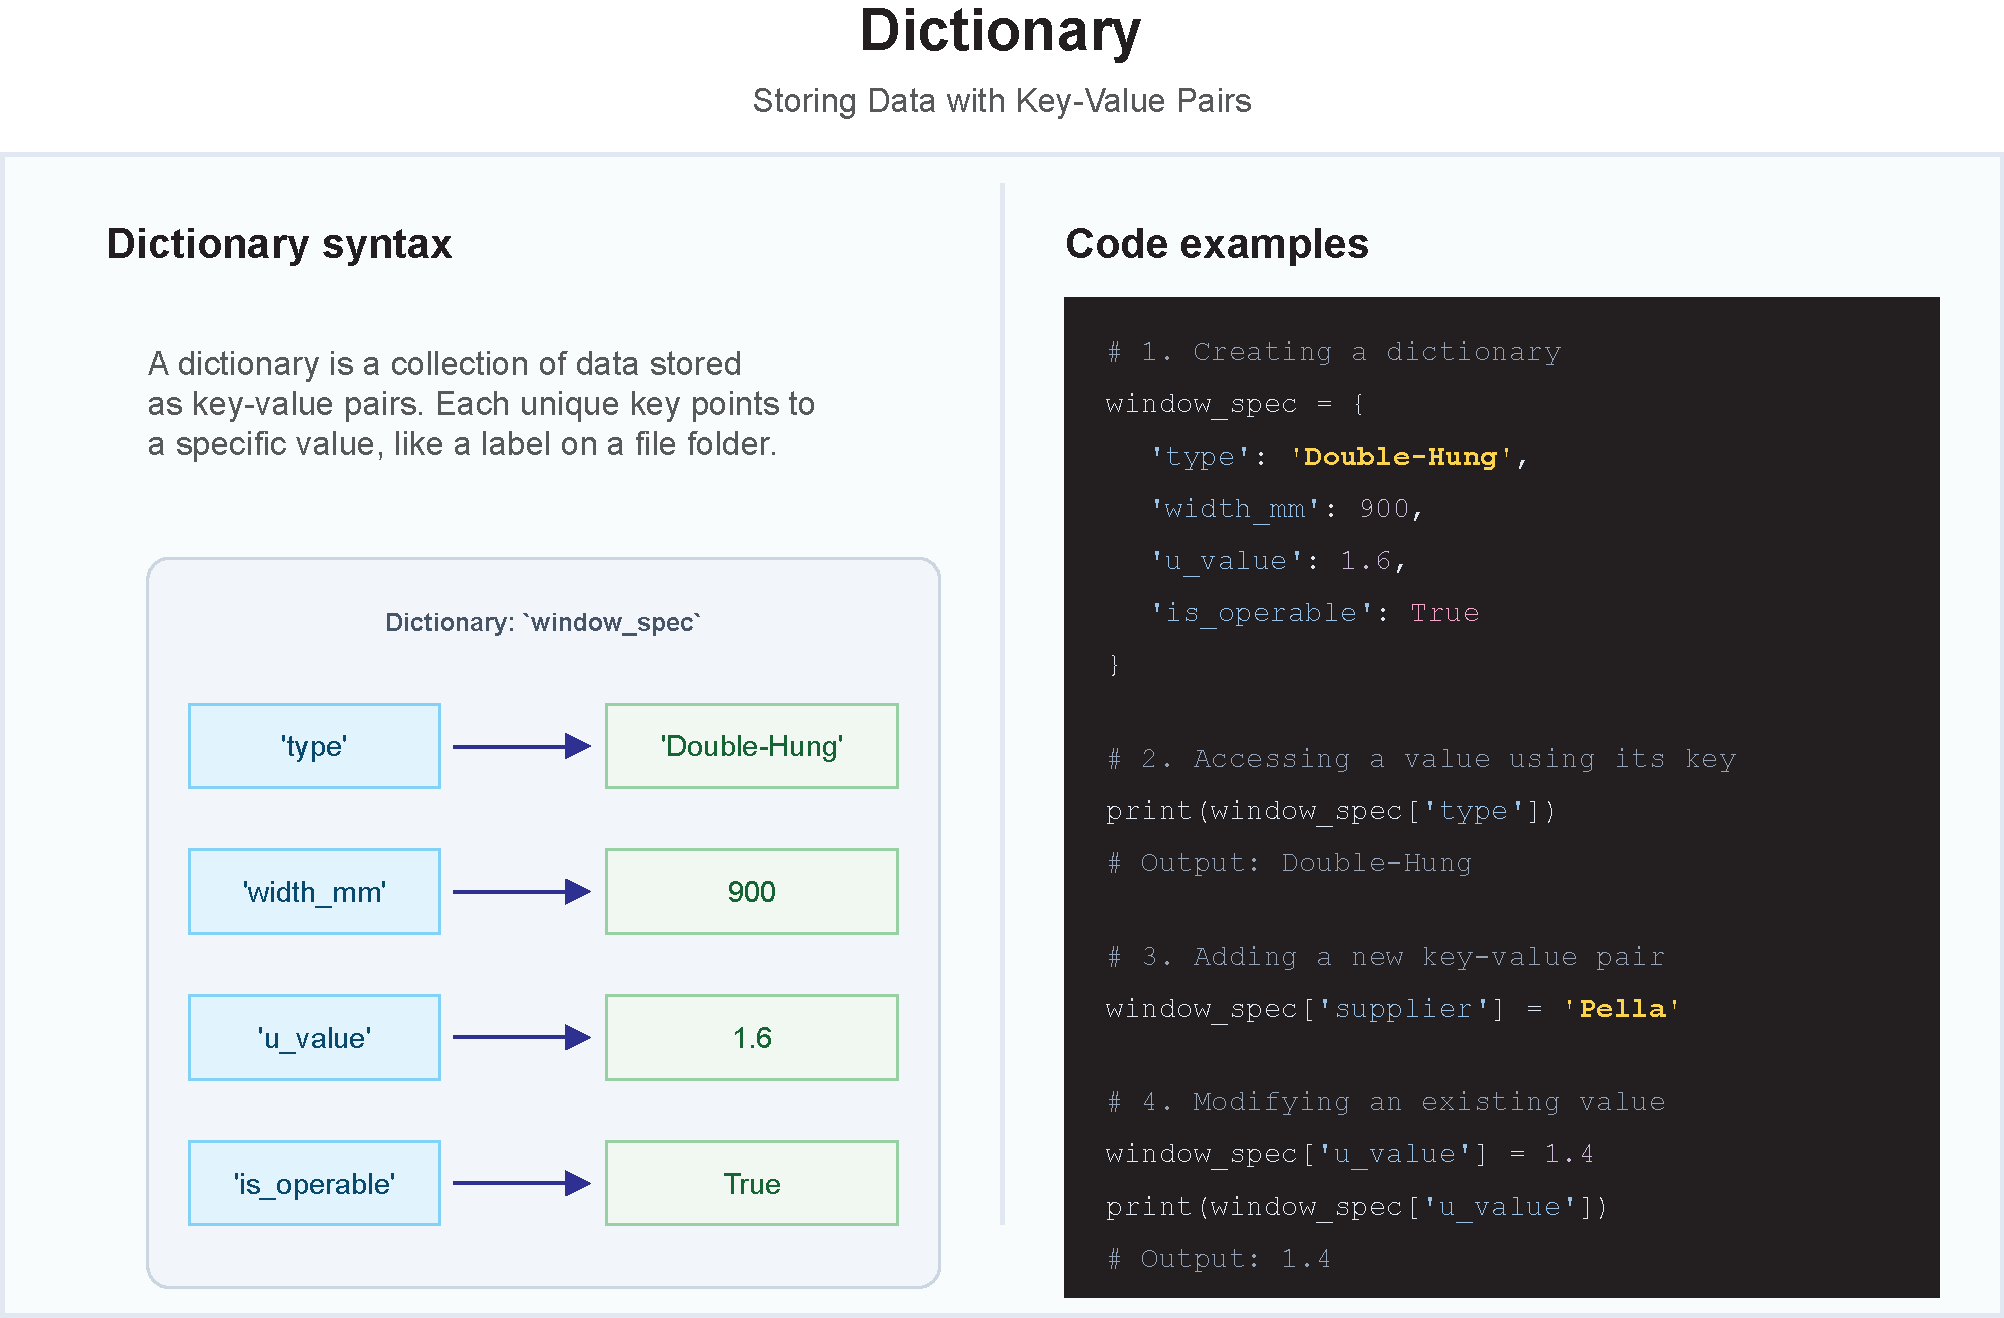
\includegraphics[width=0.85\linewidth]{Figures/Dictionary/Dictionary.pdf}
    \caption{Dictionary syntax and example}
    \label{fig:dictionary}
\end{figure}
\hh{General Syntax}
A dictionary literal uses curly braces with \c{key: value} pairs. Access values by key; update by assigning to a key.

\textit{Key syntax.}
\begin{itemize}
  \item Literal: \c{{key1: value1, key2: value2}} \quad (empty: \c{{}})
  \item Access: \c{d[key]} \quad Safe access: \c{d.get(key, default)}
  \item Insert / Update: \c{d[key] = value}, \c{d.update(\{k: v\})}
  \item Remove: \c{del d[key]}, \c{d.pop(key[, default])}, \c{d.clear()}
  \item Iterate: \c{d.keys()}, \c{d.values()}, \c{d.items()}
  \item Merge: \c{d1 | d2} (new dict, Py 3.9+), \c{d1.update(d2)} (in place)
\end{itemize}

\code{c06_dict_general}{python}{
    # General syntax of a dictionary:
    # dictionary_name = { key1: value1, key2: value2, ... }

    # A tiny dictionary
    room = {"code": "A-101", "area_m2": 18.5}
    print(room)   
    # Outcome: {'code': 'A-101', 'area_m2': 18.5}

    # Example 1: Room areas (key = room name, value = area in m²)
    room_area = {"Lobby": 120, "Studio": 200, "Office": 150}
    print(room_area)
    # Outcome: {'Lobby': 120, 'Studio': 200, 'Office': 150}

    # Example 2: Material costs (key = material, value = cost per m²)
    material_cost = {"Carpet": 15, "Tile": 20, "Wood": 25}
    print(material_cost["Tile"])
    # Outcome: 20

    # Example 3: Student info (mixed value types)
    student = {"Name": "Alex", "Age": 21, "Major": "Architecture"}
    print(student["Major"])
    # Outcome: Architecture
}{General dictionary literal, syntax, and examples.}

\hh{Creating and Inspecting Dictionaries}

Create a dictionary in one step with a literal, or start empty and add items as you go (useful when building from user input or files).

\textit{Key syntax.}
\begin{itemize}
  \item Create: \c{d = {"name": "Studio", "levels": 2}}
  \item Start empty: \c{d = {}; d["code"] = "A-101"}
  \item Type check: \c{type(d)} is \c{dict}
\end{itemize}

\code{c06_dict_basics}{python}{
    # Create directly with a literal
    building = {"name": "Studio", "levels": 2}
    print(building)                 
    # Outcome: {'name': 'Studio', 'levels': 2}

    # Start empty and add items step by step
    info = {}
    info["code"] = "A-101"
    info["area_m2"] = 18.5
    print(info)                     
    # Outcome: {'code': 'A-101', 'area_m2': 18.5}

    # Create with keys but placeholder values, fill later
    room = {"code": None, "area_m2": None}
    room["code"] = "B-202"
    room["area_m2"] = 22.0
    print(room)
    # Outcome: {'code': 'B-202', 'area_m2': 22.0}

    # Check type
    print(type(building))           
    # Outcome: <class 'dict'>
}{Create with a literal, add keys later, or start with placeholders.}


\hh{Accessing Data (Safe vs. Unsafe)}

\c{d[key]} retrieves a value but raises \c{KeyError} if the key is missing. \c{d.get(key, default)} returns a default (or \c{None}) instead, avoiding crashes.

\textit{Key syntax.}
\begin{itemize}
  \item Direct access: \c{d[key]}  \quad (errors if key missing)
  \item Safe access: \c{d.get(key, default)}
\end{itemize}

\code{c06_dict_access}{python}{
    building = {"name": "Studio", "levels": 2}

    # Access with [] - works if the key exists
    print(building["name"])          # Outcome: Studio

    # Access with [] - raises KeyError if missing
    # print(building["city"])        # Outcome: KeyError: 'city'

    # Access with get() - returns None if missing
    print(building.get("city"))      # Outcome: None

    # Access with get() and a default value
    print(building.get("city", "N/A"))  # Outcome: N/A
}{{[ ]} raises KeyError if missing; {get()} returns None or a default.}

\hh{Modifying Dictionaries: Insert, Update, Remove}

Assigning to a key either inserts (if new) or updates (if existing). Remove items with \c{del} or \c{pop}. \c{clear()} removes everything.

\textit{Key syntax.}
\begin{itemize}
  \item Insert/Update: \c{d[key] = value}
  \item Update many: \c{d.update({"k1": v1, "k2": v2})}
  \item Remove (delete): \c{del d[key]}
  \item Remove and return: \c{d.pop(key[, default])}
  \item Clear all: \c{d.clear()}
\end{itemize}

\code{c06_dict_update_remove}{python}{
    building = {"name": "Studio", "levels": 2}

    building["city"] = "NYC"        # Outcome: {'name': 'Studio', 'levels': 2, 'city': 'NYC'}
    building["levels"] = 3          # Outcome: {'name': 'Studio', 'levels': 3, 'city': 'NYC'}
    building.update({"city": "Boston", "floors": 5})  
    print(building)                 # Outcome: {'name': 'Studio', 'levels': 3, 'city': 'Boston', 'floors': 5}

    removed = building.pop("city")  
    print("Removed:", removed)      # Outcome: Removed: Boston
    del building["levels"]          
    print(building)                 # Outcome: {'name': 'Studio', 'floors': 5}

    building.clear()                
    print(building)                 # Outcome: {}
}{Insert, update, update many, remove, and clear basics.}
\hh{Membership and Size}

\textbf{Membership} means “is this thing inside that container?”. For dictionaries, \c{in} checks \emph{keys} by default (not values). \textbf{Size} means “how many key–value pairs are there?” and is given by \c{len(d)}.

\textit{Key syntax.}
\begin{itemize}
  \item Key membership: \c{key in d}
  \item Value membership: \c{val in d.values()}
  \item Size (number of pairs): \c{len(d)}
\end{itemize}

\code{c06_dict_membership}{python}{
    rooms = {"Office": 28.0, "Lobby": 30.0}

    print("Lobby" in rooms)         # Outcome: True
    print("Kitchen" in rooms)       # Outcome: False
    print(30.0 in rooms)            # Outcome: False
    print(30.0 in rooms.values())   # Outcome: True
    print(len(rooms))               # Outcome: 2
}{Membership checks keys; use values() for values.}

\hh{Iterating Through a Dictionary}

Loop over keys, values, or key–value pairs using \c{keys()}, \c{values()}, \c{items()}. Looping directly over \c{d} is the same as \c{d.keys()}.

\textit{Key syntax.}
\begin{itemize}
  \item Keys: \c{for k in d.keys(): ...} (or \c{for k in d: ...})
  \item Values: \c{for v in d.values(): ...}
  \item Pairs: \c{for k, v in d.items(): ...}
\end{itemize}

\code{c06_dict_iterate}{python}{
    rooms = {"Office": 28.0, "Lobby": 30.0, "Restroom": 15.5}

    for k in rooms.keys():
        print(k)                      # Outcome: Office
                                      # Outcome: Lobby
                                      # Outcome: Restroom

    for v in rooms.values():
        print(v)                      # Outcome: 28.0
                                      # Outcome: 30.0
                                      # Outcome: 15.5

    for k, v in rooms.items():
        print(f"The {k} is {v} m^2")  # Outcome: The Office is 28.0 m^2
                                      # Outcome: The Lobby is 30.0 m^2
                                      # Outcome: The Restroom is 15.5 m^2
}{keys(), values(), items() in loops.}

\hh{Sorting Dictionary Views}

Dictionaries themselves aren’t “sorted”, but you can get \emph{sorted lists} of keys or items. Use \c{sorted()} with an optional \c{key=} function and \c{reverse=True} for descending order.

\textit{Key syntax.}
\begin{itemize}
  \item Sort keys: \c{sorted(d)} \quad (returns a new list of keys)
  \item Sort items by value: \c{sorted(d.items(), key=lambda kv: kv[1])}
  \item Descending: add \c{reverse=True}
\end{itemize}

\code{c06_dict_sort}{python}{
    areas = {"A-103": 17.2, "A-101": 18.5, "A-102": 21.0}

    # Sort keys (default: ascending order)
    print(sorted(areas))    # Outcome: ['A-101', 'A-102', 'A-103']

    # Sort items by value (largest area first)
    by_area = sorted(areas.items(), key=lambda kv: kv[1], reverse=True)
    print(by_area)          # Outcome: [('A-102', 21.0), ('A-101', 18.5), ('A-103', 17.2)]
}{Use {sorted()} on keys or items with {key=lambda}.}

\hh{Dictionary Comprehensions}

Build a new dictionary from an iterable in one line, optionally filtering or transforming entries.

\textit{Key syntax.}
\begin{itemize}
  \item Pattern: \c{{k\_expr: v\_expr for k, v in iterable if condition}}
\end{itemize}

\code{c06_dict_comp}{python}{
    areas = {"A-101": 18.5, "A-102": 21.0, "A-103": 17.2}

    big = {k: v for k, v in areas.items() if v >= 20.0}
    print(big)                      # -> {'A-102': 21.0}

    sqft = {k: round(v * 10.764, 1) for k, v in areas.items()}
    print(sqft)                     # -> {'A-101': 199.1, 'A-102': 226.0, 'A-103': 185.1}
}{Filter or transform while building a new dict.}

\hh{Merging and Copying}

Combine multiple dictionaries or make a new independent copy. The union operator \c{|} (Py 3.9+) creates a new merged dict; \c{update()} merges in place. \c{copy()} makes a shallow copy (new object).

\textit{Key syntax.}
\begin{itemize}
  \item New merged dict (Py 3.9+): \c{d = d1 | d2}
  \item In-place merge: \c{d1.update(d2)}
  \item Shallow copy: \c{d.copy()}
\end{itemize}

\hhh{Merging}

\code{c06_dict_merge}{python}{
    dims_w = {"width": 5.0}
    dims_l = {"length": 6.0}

    rect = dims_w | dims_l
    print(rect)                     # -> {'width': 5.0, 'length': 6.0}

    dims_w.update({"height": 3.0})
    print(dims_w)                   # -> {'width': 5.0, 'height': 3.0}
}{Merge with | (new dict) or update() (in place).}

\hhh{Copying}

\code{c06_dict_copy}{python}{
    original = {"name": "Studio", "levels": 2}

    cpy = original.copy()           # shallow copy (new dict)
    cpy["name"] = "Annex"

    print(original)                 # -> {'name': 'Studio', 'levels': 2}
    print(cpy)                      # -> {'name': 'Annex', 'levels': 2}
}{copy() makes a new (shallow) dictionary.}

\hh{Advanced: Dictionaries with List or Combined Values}

A dictionary value does not have to be a single number or string.  
It can be a list, tuple, or even another dictionary.  
This allows one key to represent multiple related values.

\hhh{Values as Lists}

\code{c06_dict_list_values}{python}{
    rooms = {
        "Lobby": ["Reception desk", "Sofa", "Elevator"],
        "Studio": ["Desks", "Storage", "Projector"],
        "Office": ["Chair", "Bookshelf"]
    }

    print(rooms["Studio"])          # Outcome: ['Desks', 'Storage', 'Projector']
    print(rooms["Studio"][0])       # Outcome: Desks

    # Add a new furniture item
    rooms["Office"].append("Printer")
    print(rooms["Office"])          # Outcome: ['Chair', 'Bookshelf', 'Printer']
}{Dictionary values can be lists.}
 
\hhh{Combining Values with Tuples}

Values can also be **tuples** or more complex structures.  
For example, each room could store both its area and a list of furniture.

\code{c06_dict_combo_values}{python}{
    building = {
        "Lobby": (30.0, ["Reception desk", "Sofa"]),
        "Studio": (45.5, ["Desks", "Projector"]),
        "Office": (25.0, ["Chair", "Bookshelf", "Printer"])
    }

    # Access area
    print(building["Lobby"][0])     # Outcome: 30.0
    # Access furniture list
    print(building["Lobby"][1])     # Outcome: ['Reception desk', 'Sofa']
}{A tuple holds multiple values for each key.}

\hhh{Sorting by Complex Values}

When values are lists or tuples, you can use \c{sorted()} with a custom \c{key} function.  

\textit{Example:} Sort rooms by area (the first item in the tuple).

\code{c06_dict_sort_combo}{python}{
    building = {
        "Lobby": (30.0, ["Reception desk", "Sofa"]),
        "Studio": (45.5, ["Desks", "Projector"]),
        "Office": (25.0, ["Chair", "Bookshelf", "Printer"])
    }

    # Sort by area (tuple[0])
    by_area = sorted(building.items(), key=lambda kv: kv[1][0], reverse=True)
    print(by_area)
    # Outcome: [('Studio', (45.5, ['Desks', 'Projector'])),
    #           ('Lobby', (30.0, ['Reception desk', 'Sofa'])),
    #           ('Office', (25.0, ['Chair', 'Bookshelf', 'Printer']))]
}{Sort dictionary items by tuple values.}

\hh{Mini-Lab A: Room Directory Builder}
\begin{itemize}
  \item Create an empty dictionary \c{rooms}.
  \item Insert three rooms with areas.
  \item Update one area; remove one room; check membership and size.
  \item Print a simple report of remaining rooms.
\end{itemize}

\code{c06_minilab_a}{python}{
    rooms = {}                                   # start empty
    rooms["Lobby"] = 30.0
    rooms["Office"] = 28.0
    rooms["Studio"] = 64.0
    print(rooms)                                 # -> {'Lobby': 30.0, 'Office': 28.0, 'Studio': 64.0}

    rooms["Office"] = 29.0                       # update
    removed = rooms.pop("Lobby")                 # remove + return
    print("Removed:", removed)                   # -> Removed: 30.0

    print("Studio" in rooms, len(rooms))         # -> True 2

    for k, v in rooms.items():                   # simple report
        print(f"{k}: {v} m^2")                   # -> Office: 29.0 m^2 / Studio: 64.0 m^2
}{Build, update, remove, and report.}

\hh{Mini-Lab B: Sorted Material Costs}
\begin{itemize}
  \item Given \c{cost = {"steel": 2.2, "glass": 1.8, "concrete": 1.4}} (cost per unit).
  \item Print materials sorted by cost (ascending).
  \item Make a new dictionary with a 10\% markup using a comprehension.
\end{itemize}

\code{c06_minilab_b}{python}{
    cost = {"steel": 2.2, "glass": 1.8, "concrete": 1.4}

    by_cost = sorted(cost.items(), key=lambda kv: kv[1])
    print(by_cost)                                # -> [('concrete', 1.4), ('glass', 1.8), ('steel', 2.2)]

    with_markup = {k: round(v * 1.10, 2) for k, v in cost.items()}
    print(with_markup)                            # -> {'steel': 2.42, 'glass': 1.98, 'concrete': 1.54}
}{Sort items by value; transform with a comprehension.}

\hh{Key Takeaways}
\begin{tcolorbox}[% passing options here
    colframe=orange,
    colback = white,
%    colback=orange!40!yellow!30, % think of mixing 2 colors with sliders
    arc=2mm % sharp corners
 ]
\begin{itemize}
  \item A dictionary maps \textbf{unique keys} to \textbf{values}; use it when labels matter more than positions.
  \item Use \c{d[key]} when you \emph{know} the key exists; prefer \c{d.get(key, default)} when it might not.
  \item Insert/update with \c{d[key] = value} (single) or \c{update()} (multiple).
  \item Remove with \c{del d[key]} or \c{pop(key)}; \c{clear()} empties the dict.
  \item \c{in} checks \emph{keys}; use \c{values()} to check values. \c{len(d)} gives the number of pairs.
  \item Iterate with \c{keys()}, \c{values()}, \c{items()} depending on what you need.
  \item Dictionaries aren’t sorted; use \c{sorted()} on keys/items with \c{key=} and \c{reverse=True}.
  \item Comprehensions create filtered/transformed dictionaries succinctly.
  \item Merge with \c{|} (new dict) or \c{update()} (in place); \c{copy()} creates a shallow copy.
\end{itemize}
\end{tcolorbox}